\rev{\section{Extraction Performance}} \label{sec: Extraction Performance}

\rev{\textbf{Experimental Setup.}} Clinical note mining for rare disease differential diagnosis involves two key tasks: extracting phenotypes and identifying rare diseases. \rev{Here, we summarize the experimental setup towards evaluating existing mining approaches and RDMA.}

\textbf{Datasets.} \rev{Existing rare disease datasets have known limitations but remain useful benchmarks. Phenotype identification. We evaluate on the case study cohort (CSC) \cite{garcia2024_HPORAG} and BioLark gold standard corpora \cite{yang2023enhancingphenotyperecognitionclinical}. The CSC benchmark better reflects clinical notes with more text and phenotypes per document, though it still falls short of real-world clinical complexity. Rare disease identification. Three benchmarks exist: RDD \cite{fabregat2018deep_rdd}, RareDis \cite{martinez2022raredis}, and a noisily annotated MIMIC-III disease benchmark \cite{johnson2016mimic3,dong2023ontology_poor_annotations}. We exclude RDD as it lacks rare disease mention annotations. To demonstrate RDMA's ability to both improve extraction and assist annotators, we construct a gold evaluation set from the MIMIC-III annotations via combined human and agent annotation, yielding a realistic benchmark on real clinical notes. All benchmark statistics are described in Supplementary Table~\sTabDatasets.}

\rev{\textbf{Evaluation.} Our goal is to map text evidence to structured codes from the HPO \cite{gargano2024mode_hpo} and Orphanet \cite{weinreich2008orphanet} ontologies, framing extraction as a medical coding task \cite{Edin_2023_medical_coding_review}. Phenotype extraction. Annotated codes are available for both phenotype datasets, making evaluation straightforward. Rare disease identification. RareDis provides only text span annotations without ontology mappings. As both exist in our MIMIC3 evaluation set, we report both span and code mapping performance here as MIMIC3-RD Entity and MIMIC3-RD Code respectively. For baselines lacking an ontology mapping step, we choose to use a fuzzy matching retrieval approach that is employed by the authors of PhenoGPT \cite{yang2023enhancingphenotyperecognitionclinical}.} All evaluation metrics are described in the Supplementary Material.


\textbf{Baselines.} \rev{Across all benchmarks, approaches fall into three categories: (1) rule-based methods that tokenize text and match to ontologies via nearest-neighbor search, (2) fine-tuned encoder models trained to extract entities directly, and (3) LLM-based methods using zero-shot or RAG-based extract-and-match pipelines.
For rule-based approaches, we include a simple retrieve-and-string-match Dictionary Match baseline using state-of-the-art clinical embeddings MedEmbed \cite{balachandran2024medembed} and the state-of-the-art FastHPOCR. For fine-tuned encoders, we distinguish between off-the-shelf models and those we fine-tune ourselves. Off-the-shelf, we evaluate PhenoGPT \cite{yang2023enhancingphenotyperecognitionclinical} and Stanza's i2b2 Clinical BERT, both used without modification. Following the RareDis authors \cite{segura2022exploring_raredis}, we additionally fine-tune BioBERT \cite{sun2021biomedical_biobert_ner} and BioClinicalBERT \cite{alsentzer2019publiclyavailableclinicalbert} for rare disease and phenotype extraction; all four encoder models are evaluated across all benchmark datasets. For LLM-based approaches, we test a range of models in both zero-shot and RAG-based settings \cite{garcia2024_HPORAG}. We note that highly specialized approaches such as FastHPOCR and PhenoGPT do not apply to our rare disease extraction benchmarks.}
\rev{\textbf{We evaluate mining performance along two axes: generalization across distributions and scaling across model sizes in Table \ref{tab:main_results_combined_v3} and Fig. \ref{fig:rd_model_perf_across_sizes}.} Specifically, we ask (1) how well does each approach generalize across benchmarks with different data characteristics, and (2) how does performance scale with model size. We find that (1) our agentic system is substantially more robust than competing approaches, outperforming specialized baselines without requiring any training, and (2) a small quantized model is sufficient for maximal performance across all benchmarks, making RDMA computationally feasible compared to LLM-based approaches that depend on larger models for robust performance.}

\begin{table}[h]
  \centering
  \small
  \setlength{\tabcolsep}{3.5pt}
  \renewcommand{\arraystretch}{1.18}
  \resizebox{\textwidth}{!}{%
  \begin{tabular}{l c ccc ccc ccc ccc ccc}
    \toprule
    & & \multicolumn{6}{c}{\textbf{Phenotype Mining}} & \multicolumn{9}{c}{\textbf{Rare Disease Mining}} \\
    \cmidrule(lr){3-8} \cmidrule(lr){9-17}
    & & \multicolumn{3}{c}{\textbf{BiolarkGSC+}} & \multicolumn{3}{c}{\textbf{CSC}} & \multicolumn{3}{c}{\textbf{RareDis}} & \multicolumn{3}{c}{\textbf{MIMIC3-RD Entity}} & \multicolumn{3}{c}{\textbf{MIMIC3-RD Code}} \\
    \cmidrule(lr){3-5} \cmidrule(lr){6-8} \cmidrule(lr){9-11} \cmidrule(lr){12-14} \cmidrule(lr){15-17}
    \textbf{Approach} & \textbf{FT} & \textbf{P} & \textbf{R} & \textbf{F1} & \textbf{P} & \textbf{R} & \textbf{F1} & \textbf{P} & \textbf{R} & \textbf{F1} & \textbf{P} & \textbf{R} & \textbf{F1} & \textbf{P} & \textbf{R} & \textbf{F1} \\
    \midrule

    \multicolumn{17}{l}{\textit{Non-LLM Baselines}} \\[1pt]
    Dictionary Match & {\color{green}\xmark} & \cellcolor[rgb]{1.000,0.574,0.054}0.682 & \cellcolor[rgb]{1.000,0.829,0.620}0.214 & \cellcolor[rgb]{1.000,0.757,0.459}0.326 & \cellcolor[rgb]{1.000,0.599,0.110}0.600 & \cellcolor[rgb]{1.000,0.859,0.687}0.210 & \cellcolor[rgb]{1.000,0.788,0.528}0.310 & \cellcolor[rgb]{1.000,0.579,0.065}0.850 & \cellcolor[rgb]{1.000,1.000,1.000}0.410 & \cellcolor[rgb]{1.000,0.752,0.448}0.550 & \cellcolor[rgb]{1.000,0.653,0.229}0.400 & \cellcolor[rgb]{1.000,1.000,1.000}0.468 & \cellcolor[rgb]{1.000,0.677,0.281}\underline{0.431} & \cellcolor[rgb]{1.000,0.707,0.349}0.300 & \cellcolor[rgb]{1.000,0.690,0.312}0.450 & \cellcolor[rgb]{1.000,0.695,0.322}\underline{0.360} \\

    FastHPOCR & {\color{green}\xmark} & \cellcolor[rgb]{1.000,0.550,0.000}0.721 & \cellcolor[rgb]{1.000,0.586,0.080}0.518 & \cellcolor[rgb]{1.000,0.550,0.000}\textbf{0.603} & \cellcolor[rgb]{1.000,0.653,0.228}0.520 & \cellcolor[rgb]{1.000,0.698,0.329}0.450 & \cellcolor[rgb]{1.000,0.671,0.269}0.480 & \multicolumn{3}{c}{\cellcolor[gray]{0.95}\textcolor{red!80}{\textit{N/A}}} & \multicolumn{3}{c}{\cellcolor[gray]{0.95}\textcolor{red!80}{\textit{N/A}}} & \multicolumn{3}{c}{\cellcolor[gray]{0.95}\textcolor{red!80}{\textit{N/A}}} \\

    i2b2 Clinical BERT & {\color{red}\cmark} & \cellcolor[rgb]{1.000,0.626,0.169}0.599 & \cellcolor[rgb]{1.000,0.667,0.259}0.417 & \cellcolor[rgb]{1.000,0.634,0.186}0.491 & \cellcolor[rgb]{1.000,0.680,0.288}0.480 & \cellcolor[rgb]{1.000,0.598,0.106}0.600 & \cellcolor[rgb]{1.000,0.637,0.193}0.530 & \cellcolor[rgb]{1.000,0.987,0.970}0.153 & \cellcolor[rgb]{1.000,0.588,0.083}0.850 & \cellcolor[rgb]{1.000,0.977,0.948}0.260 & \cellcolor[rgb]{1.000,1.000,1.000}0.010 & \cellcolor[rgb]{1.000,0.550,0.000}0.879 & \cellcolor[rgb]{1.000,1.000,1.000}0.020 & \cellcolor[rgb]{1.000,0.991,0.980}0.010 & \cellcolor[rgb]{1.000,0.550,0.000}0.651 & \cellcolor[rgb]{1.000,0.986,0.968}0.019 \\

    BioBERT$^\dagger$ & {\color{red}\cmark} & \cellcolor[rgb]{1.000,0.604,0.119}0.635 & \cellcolor[rgb]{1.000,0.673,0.274}0.409 & \cellcolor[rgb]{1.000,0.628,0.174}0.498 & \cellcolor[rgb]{1.000,0.590,0.089}0.614 & \cellcolor[rgb]{1.000,0.814,0.586}0.278 & \cellcolor[rgb]{1.000,0.738,0.419}0.382 & \cellcolor[rgb]{1.000,0.627,0.171}0.730 & \cellcolor[rgb]{1.000,0.653,0.228}0.703 & \cellcolor[rgb]{1.000,0.620,0.153}\underline{0.716} & \cellcolor[rgb]{1.000,0.993,0.984}0.018 & \cellcolor[rgb]{1.000,0.900,0.779}0.559 & \cellcolor[rgb]{1.000,0.990,0.977}0.033 & \cellcolor[rgb]{1.000,0.976,0.948}0.025 & \cellcolor[rgb]{1.000,0.674,0.276}0.473 & \cellcolor[rgb]{1.000,0.962,0.915}0.047 \\

    BioClinicalBERT$^\dagger$ & {\color{red}\cmark} & \cellcolor[rgb]{1.000,0.714,0.363}0.459 & \cellcolor[rgb]{1.000,0.661,0.247}0.424 & \cellcolor[rgb]{1.000,0.671,0.269}0.441 & \cellcolor[rgb]{1.000,0.700,0.334}0.449 & \cellcolor[rgb]{1.000,0.767,0.481}0.348 & \cellcolor[rgb]{1.000,0.732,0.403}0.392 & \cellcolor[rgb]{1.000,0.650,0.233}0.681 & \cellcolor[rgb]{1.000,0.690,0.314}0.666 & \cellcolor[rgb]{1.000,0.660,0.255}0.673 & \cellcolor[rgb]{1.000,0.996,0.990}0.015 & \cellcolor[rgb]{1.000,0.995,0.988}0.473 & \cellcolor[rgb]{1.000,0.994,0.988}0.027 & \cellcolor[rgb]{1.000,0.975,0.946}0.026 & \cellcolor[rgb]{1.000,0.637,0.193}0.527 & \cellcolor[rgb]{1.000,0.959,0.909}0.050 \\

    \midrule
    \multicolumn{17}{l}{\textit{LLM-based Approaches}} \\[1pt]

    PhenoGPT & {\color{red}\cmark} & \cellcolor[rgb]{1.000,0.578,0.062}0.676 & \cellcolor[rgb]{1.000,0.751,0.446}0.312 & \cellcolor[rgb]{1.000,0.681,0.292}0.427 & \cellcolor[rgb]{1.000,0.619,0.154}0.570 & \cellcolor[rgb]{1.000,0.738,0.419}0.390 & \cellcolor[rgb]{1.000,0.685,0.300}0.460 & \multicolumn{3}{c}{\cellcolor[gray]{0.95}\textcolor{red!80}{\textit{N/A}}} & \multicolumn{3}{c}{\cellcolor[gray]{0.95}\textcolor{red!80}{\textit{N/A}}} & \multicolumn{3}{c}{\cellcolor[gray]{0.95}\textcolor{red!80}{\textit{N/A}}} \\

    Zero-Shot (Llama 3.3 70B) & {\color{green}\xmark} & \cellcolor[rgb]{1.000,1.000,1.000}0.000 & \cellcolor[rgb]{1.000,1.000,1.000}0.000 & \cellcolor[rgb]{1.000,1.000,1.000}0.000 & \cellcolor[rgb]{1.000,1.000,1.000}0.000 & \cellcolor[rgb]{1.000,1.000,1.000}0.000 & \cellcolor[rgb]{1.000,1.000,1.000}0.000 & \cellcolor[rgb]{1.000,0.550,0.000}0.900 & \cellcolor[rgb]{1.000,0.850,0.667}0.570 & \cellcolor[rgb]{1.000,0.635,0.190}0.700 & \cellcolor[rgb]{1.000,0.883,0.741}0.141 & \cellcolor[rgb]{1.000,0.853,0.674}0.602 & \cellcolor[rgb]{1.000,0.836,0.636}0.228 & \cellcolor[rgb]{1.000,1.000,1.000}0.001 & \cellcolor[rgb]{1.000,1.000,1.000}0.007 & \cellcolor[rgb]{1.000,1.000,1.000}0.002 \\

    RAG (RD / HPO) (Llama 3.3 70B) & {\color{green}\xmark} & \cellcolor[rgb]{1.000,0.744,0.431}0.410 & \cellcolor[rgb]{1.000,0.550,0.000}0.563 & \cellcolor[rgb]{1.000,0.646,0.212}0.475 & \cellcolor[rgb]{1.000,0.550,0.000}0.674 & \cellcolor[rgb]{1.000,0.611,0.136}0.580 & \cellcolor[rgb]{1.000,0.573,0.050}\underline{0.624} & \cellcolor[rgb]{1.000,1.000,1.000}0.130 & \cellcolor[rgb]{1.000,0.550,0.000}0.890 & \cellcolor[rgb]{1.000,1.000,1.000}0.230 & \cellcolor[rgb]{1.000,0.969,0.931}0.045 & \cellcolor[rgb]{1.000,0.728,0.397}0.716 & \cellcolor[rgb]{1.000,0.949,0.886}0.085 & \cellcolor[rgb]{1.000,0.984,0.965}0.017 & \cellcolor[rgb]{1.000,0.607,0.126}0.570 & \cellcolor[rgb]{1.000,0.976,0.947}0.030 \\

    \textbf{RDMA (Mistral 24B)}$^{\ast}$ & {\color{green}\xmark} & \cellcolor[rgb]{1.000,0.647,0.216}0.565 & \cellcolor[rgb]{1.000,0.558,0.018}0.553 & \cellcolor[rgb]{1.000,0.583,0.073}\underline{0.559} & \cellcolor[rgb]{1.000,0.570,0.045}0.644 & \cellcolor[rgb]{1.000,0.550,0.000}0.671 & \cellcolor[rgb]{1.000,0.550,0.000}\textbf{0.657} & \cellcolor[rgb]{1.000,0.568,0.039}0.870 & \cellcolor[rgb]{1.000,0.672,0.271}0.760 & \cellcolor[rgb]{1.000,0.550,0.000}\textbf{0.810} & \cellcolor[rgb]{1.000,0.550,0.000}0.516 & \cellcolor[rgb]{1.000,0.751,0.448}0.695 & \cellcolor[rgb]{1.000,0.550,0.000}\textbf{0.592} & \cellcolor[rgb]{1.000,0.550,0.000}0.460 & \cellcolor[rgb]{1.000,0.572,0.048}0.620 & \cellcolor[rgb]{1.000,0.550,0.000}\textbf{0.530} \\

    \bottomrule
  \end{tabular}%
  }
  \caption{\rev{\textbf{Standardized Performance Comparison Across Phenotype and Rare Disease Mining Approaches.} We evaluate both domains side-by-side using various LLM backbones for generative methods. For Rare Disease evaluation, BioBERT and BioClinicalBERT$^\dagger$ are fine-tuned on datasets (BiolarkGSC+, RareDis) where span annotations exist and evaluated on their evaluation counterparts (CSC, MIMIC3-RD) here. ``N/A" blocks denote models whose architectures or pre-training are not applicable to the respective dataset. Colors are normalized per benchmark so that the darkest orange always reflects the highest score within each column group. FT indicates whether the model was fine-tuned on any biomedical corpus before usage. \textbf{Bold} denotes best performance, \underline{underline} denotes second best. We report our bootstrapped confidence intervals in Appendix section \ref{appdx: CIs}. }}
  \label{tab:main_results_combined_v3}
\end{table}

\begin{figure}[h]
    \centering
    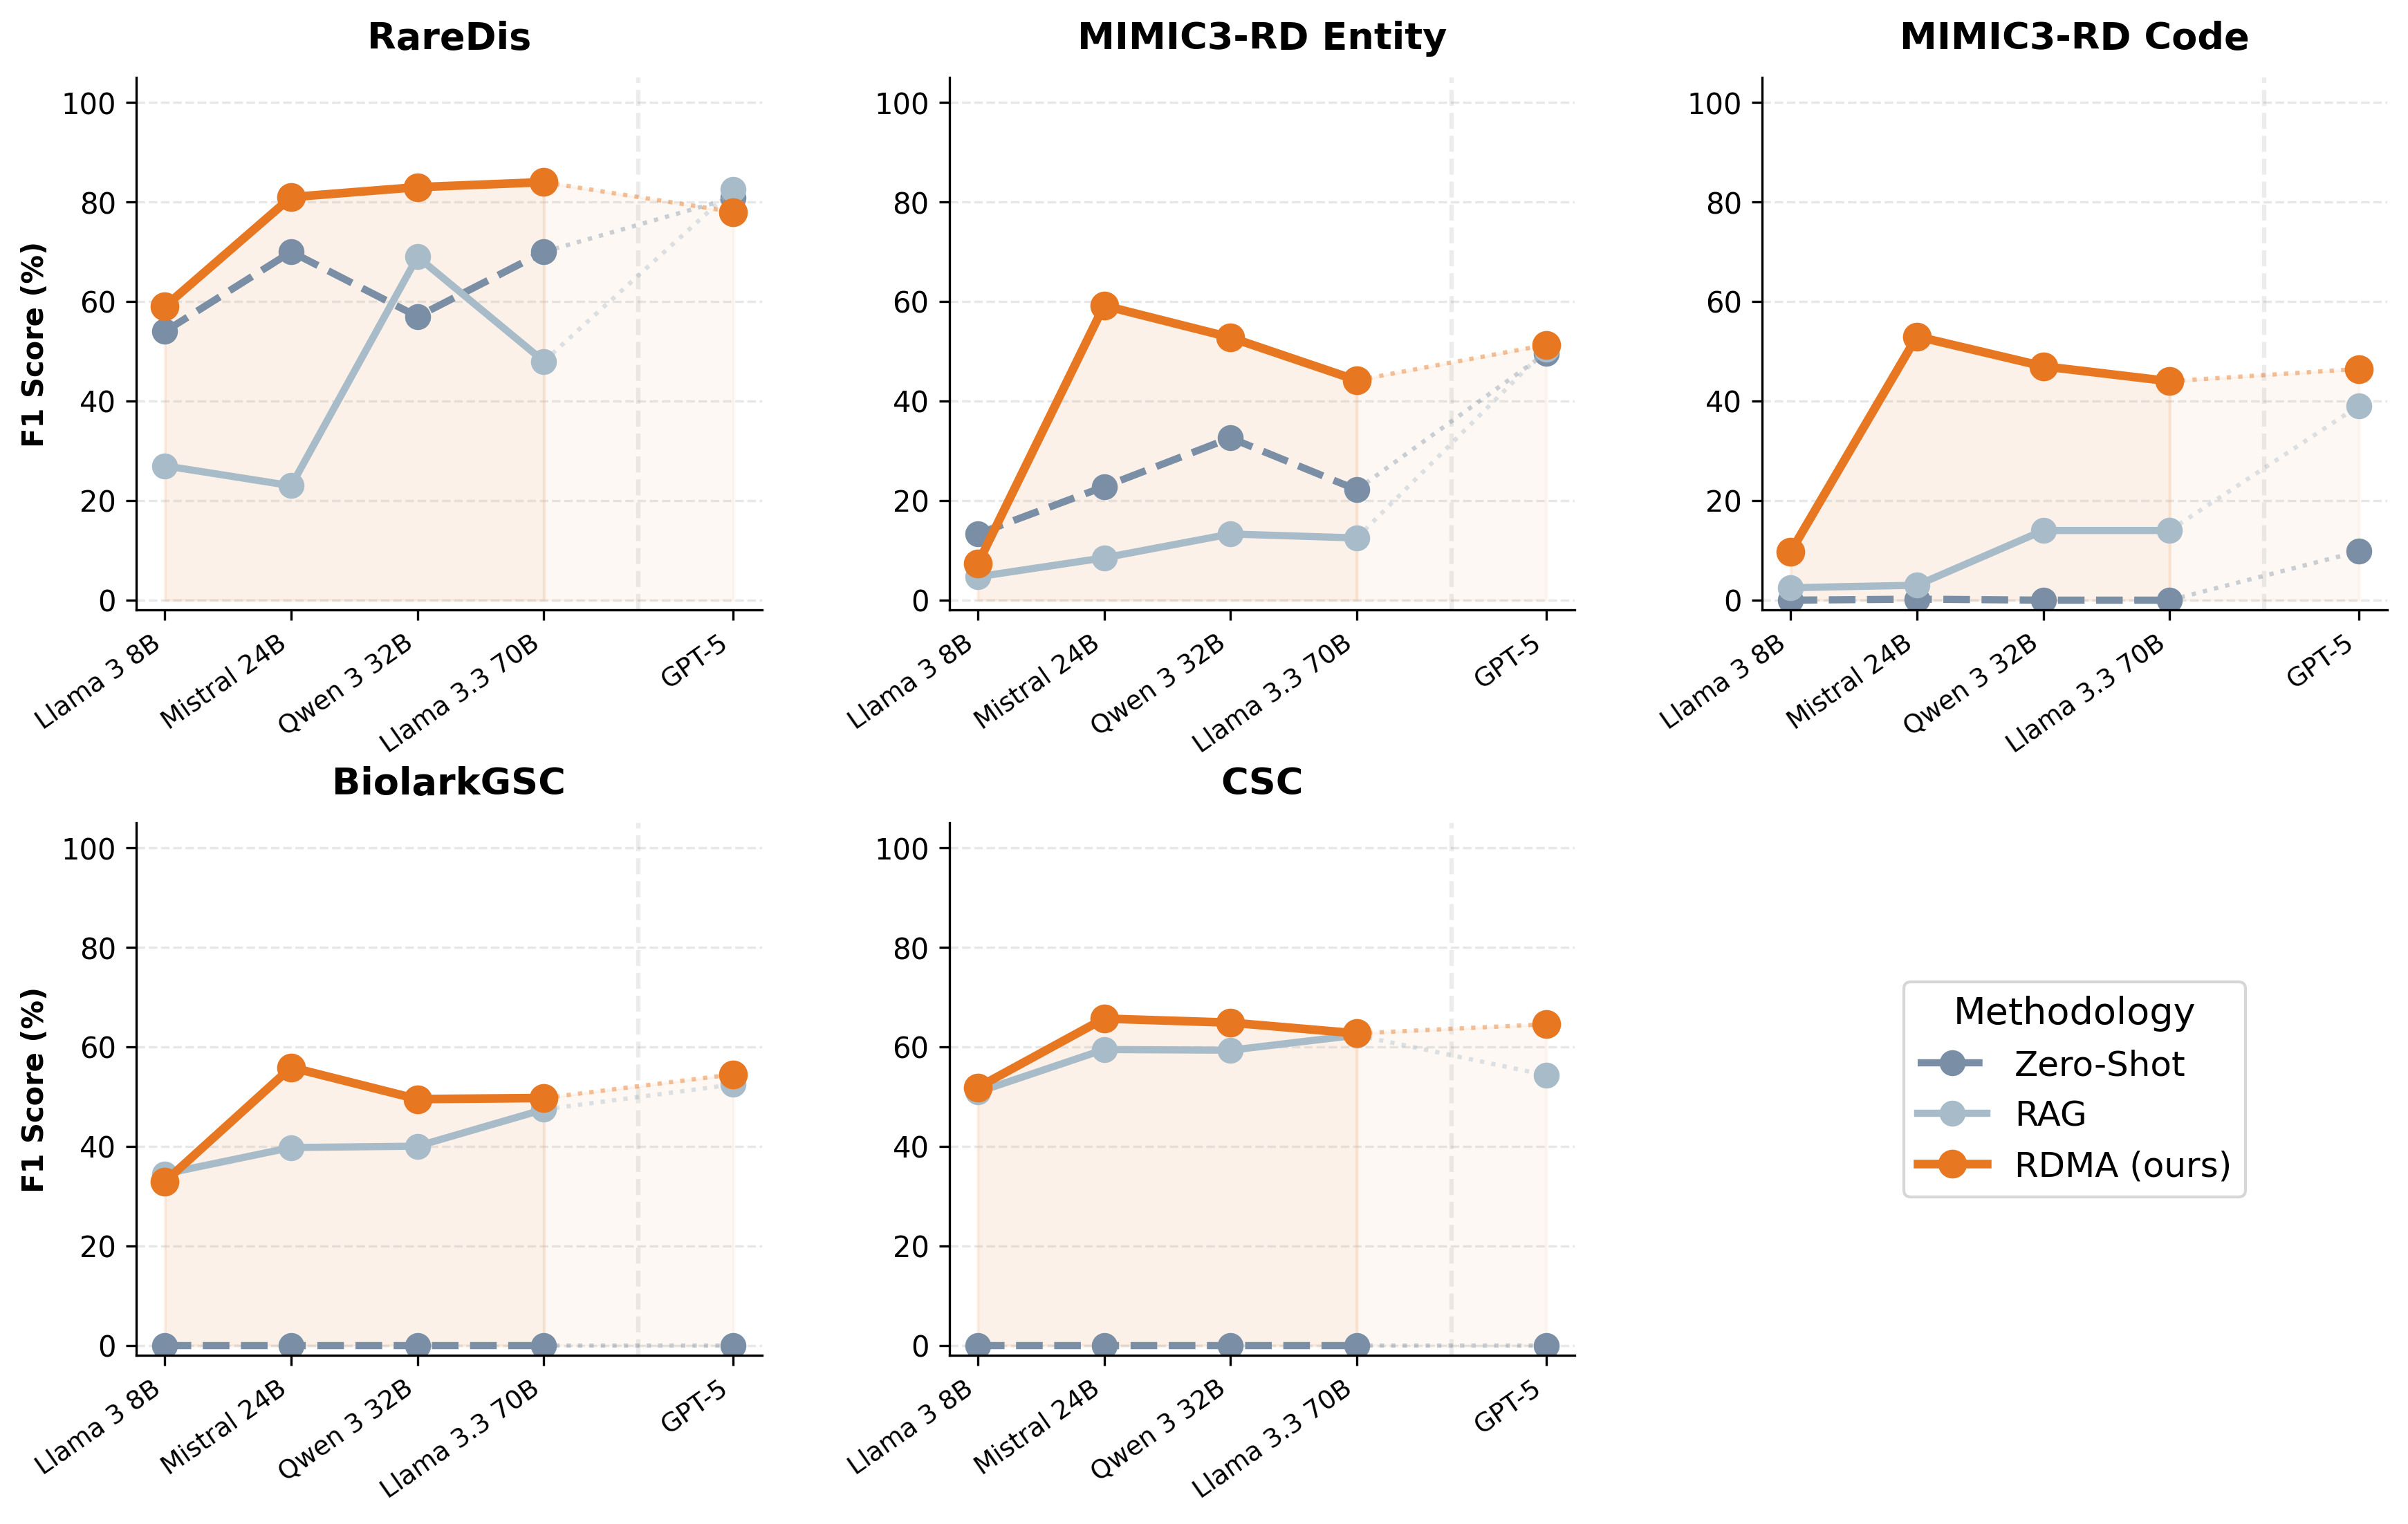
\includegraphics[width=1.0\textwidth]{figs/fig2_compact_scaling.png}
    \caption{\rev{\textbf{Performance of LLM rare disease mining performance across model sizes and approaches.} We observe that in general increasing the model sizes does not improve performance of downstream mining approaches for rare diseases beyond a certain model size and intelligence, namely the Mistral 24B model. We also observe that mining performance for baseline RAG or zero-shot approaches fluctuate dramatically as seen on the RareDis and MIMIC3-RD Entity benchmarks. }}
    \label{fig:rd_model_perf_across_sizes}
\end{figure}


\rev{\textbf{Agentic LLM approaches better generalize across distributions without domain-specific training.} For datasets where annotations do not contain explicit text spans and sample sizes are small, such as CSC and MIMIC3, fine-tuning is practically infeasible, and even where it is feasible, supervised models trained on one corpus frequently fail to generalize to out-of-distribution data. As shown in Table~\ref{tab:main_results_combined_v3}, fine-tuned models such as PhenoGPT, BioBERT, and BioClinicalBERT require extensive training on well-annotated corpora such as BiolarkGSC+ and RareDis, yet exhibit substantial performance degradation when evaluated on out-of-distribution benchmarks like CSC and MIMIC3. Rule-based approaches like FastHPOCR avoid this training requirement but exhibit similar brittleness: FastHPOCR \cite{groza2024fasthpocr} well on the benchmark it was originally evaluated on, but underperforms on CSC \cite{garcia2024_HPORAG}. By contrast, RDMA generalizes across extraction tasks without any additional training, providing a substantial performance uplift across 4 of the 5 benchmarks compared to both trained and rule-based alternatives.}

\rev{\textbf{LLMs hallucinate HPO and Orpha codes.} In benchmarks requiring both entity extraction and ontology code assignment, we observe that LLMs frequently hallucinate invalid HPO and Orpha codes despite correctly identifying the underlying text spans, as evidenced by the performance gap between text-span and code-based benchmarks in Table~\ref{tab:main_results_combined_v3}. Providing retrieved ontology context in the RAG setting substantially improves code-level performance, but often at the cost of recall as false positives increase. We hypothesize that retrieved ontology context biases the model toward over-predicting entity presence, surfacing mentions that are not actually attested in the source text.}

\rev{\textbf{Larger models do not improve extraction performance.} Beyond 8B models, which frequently struggle to follow structured instructions, we observe that increasing model size from 24B up to proprietary models such as GPT-5 yields no consistent improvement in rare disease or phenotype extraction performance across any benchmark, with gains effectively plateauing.}

\begin{wrapfigure}{r}{0.5\textwidth}
\centering
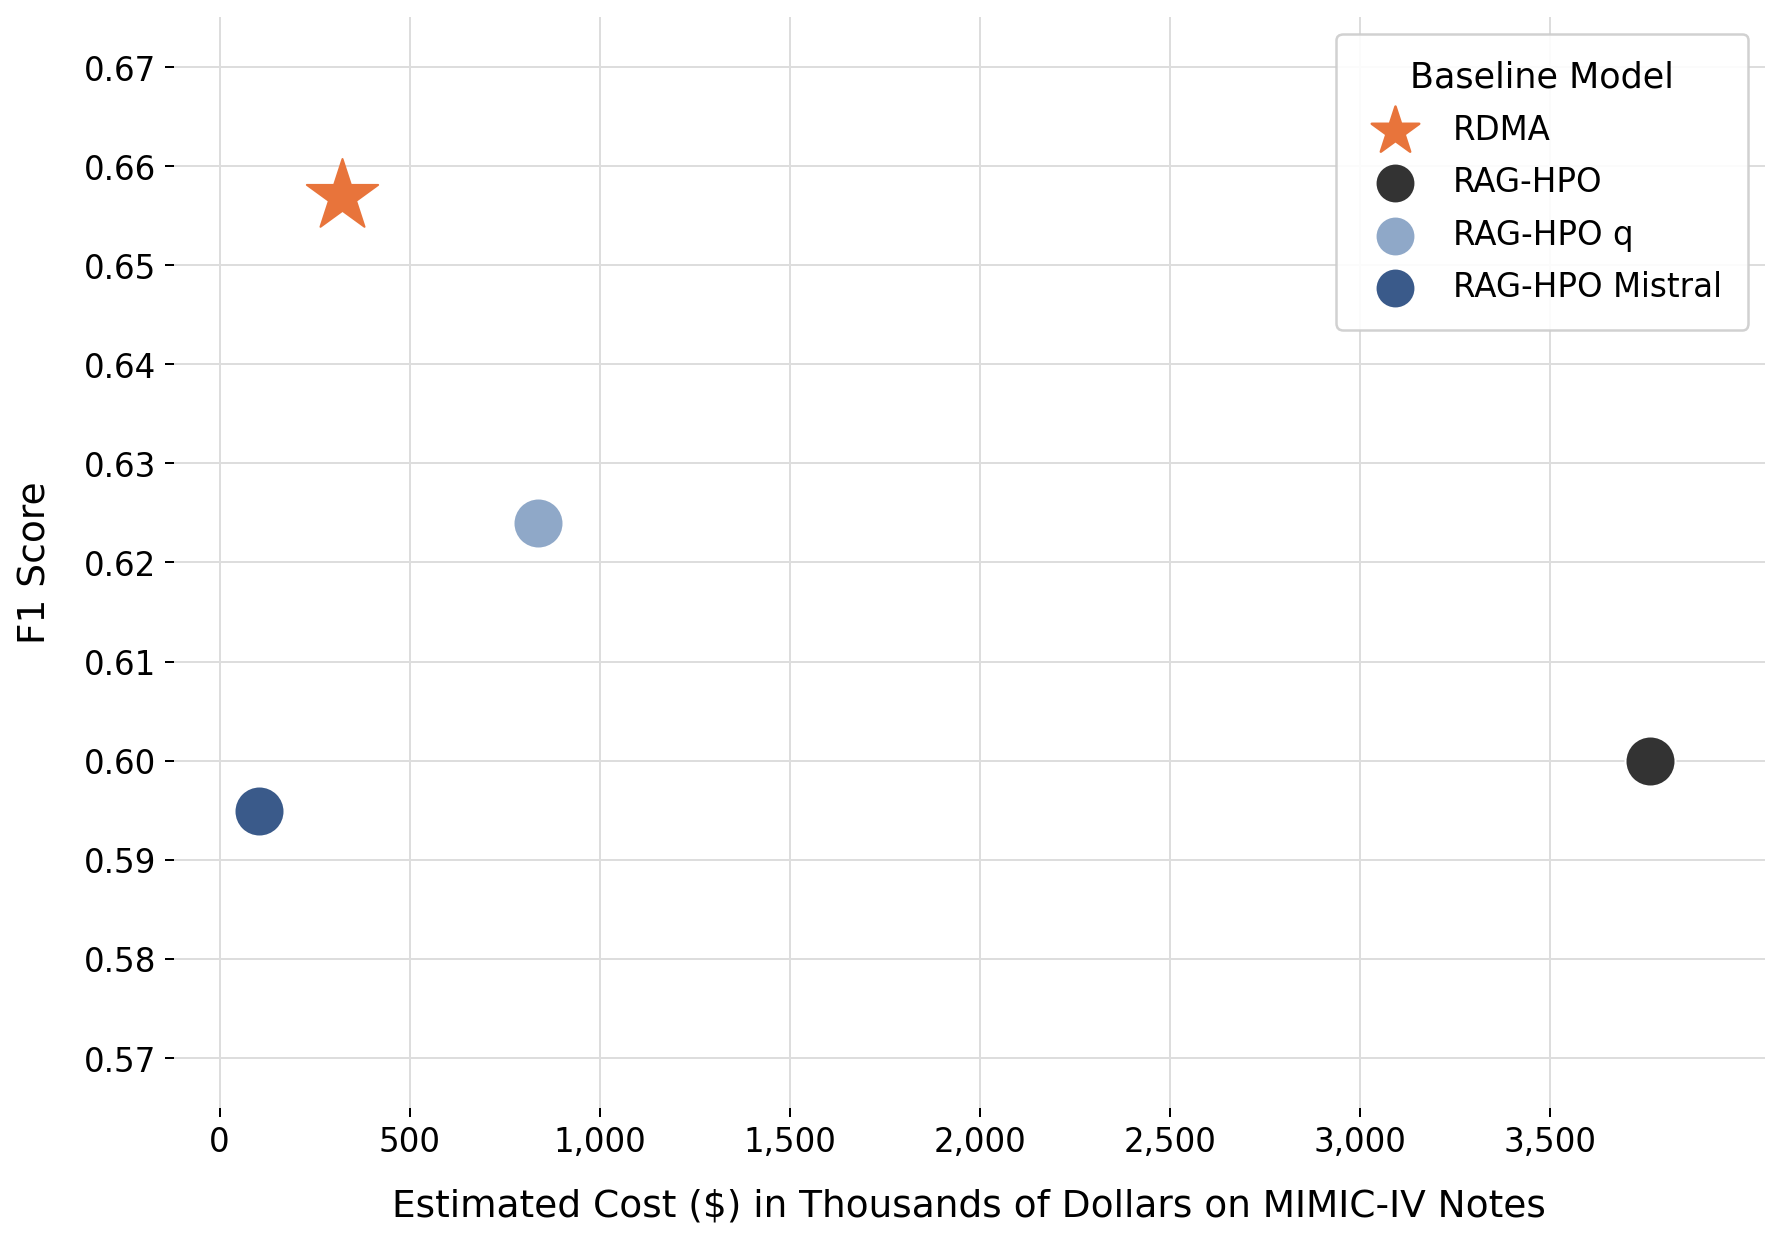
\includegraphics[width=0.5\textwidth]{figs/performance_cost_chart_updated.png}
\caption{\rev{\textbf{Phenotype mining inference costs with LLMs.} RDMA uses a 4-bit quantized Mistral 24B model yet outperforms RAG-HPO variants running on both a 4-bit and full non-quantized Llama 3.3 70B, models that are substantially more expensive to run locally. Although RDMA's additional reasoning steps incur a modest overhead when normalized by model size, this cost is far smaller than the penalty of scaling to larger models.} We use GPU rental pricing from cloud-providers \cite{salad_pricing} \cite{hyperstack_gpu_pricing} to compute our estimated inference costs in Appendix \ref{appendix: cost calculations}.}
\label{fig:performance_cost}
\end{wrapfigure}

\rev{\textbf{RDMA provides a more a stable foundation for LLM mining performance.} Different LLMs can respond very differently to the same prompts, and as shown in Fig.~\ref{fig:rd_model_perf_across_sizes}, extraction performance varies substantially across model families in both zero-shot and RAG settings on the RareDis and MIMIC3-RD Entity benchmarks. Notably, RDMA consistently achieves the highest or comparable F1 across all configurations regardless of the underlying LLM.}

\rev{\textbf{Larger models are too expensive to deploy locally on large clinical corpuses.} Estimating mining costs on MIMIC-IV notes \cite{johnson2023mimic4_note} based on run time and GPU rental prices, we observe that larger non-quantized LLMs are substantially more expensive to run (i.e up to 10x) than their smaller quantized counterparts in Fig.~\ref{fig:performance_cost}.}

\rev{\textbf{Additional reasoning steps enable smaller quantized models to surpass larger ones.} While the performance gap between RAG-based approaches and RDMA narrows as model size increases in Fig.~\ref{fig:rd_model_perf_across_sizes}, smaller models remain substantially cheaper to run. As illustrated in Fig.~\ref{fig:performance_cost}, our quantized 24B Mistral model exceeds the performance of the much larger non-quantized Llama 3.3 70B at a fraction of the cost. Moreover, as shown in Fig.~\ref{fig:rd_model_perf_across_sizes}, RDMA performance is comparable to our cloud-based GPT-5 baseline regardless of the underlying framework, suggesting that frontier models do not necessarily confer an advantage on rare disease mining tasks.}



% \textbf{Additional reasoning steps with RDMA enables smaller models to outperform much larger models at a fraction of the cost.} Compared to its RAG-based counterparts \cite{garcia2024_HPORAG}, RDMA improves recall performance by over 5\% as shown in Table \ref{tab:model_comparison}, while dramatically reducing upfront operational costs by approximately 4x. Similar to how a clinician reasons when reading clinical notes, these models must go beyond the simple extraction and matching employed in previous phenotype extraction approaches. Specifically, such models must not only extract terms but also verify the accuracy of their extractions and identify implied phenotypes not explicitly mentioned in the text. Fig. \ref{fig:performance_cost} demonstrates that RDMA outperforms all baselines while incurring only minimal additional inference costs for its reasoning steps when compared to similarly-sized RAG-HPO setups using Mistral. One key benefit of moving towards smaller models is that local hardware costs are substantially lower, meaning RDMA is more accessible to a wider range of users. Such costs are key when hospitals must run these tasks locally due to privacy concerns. Please refer to Table \ref{tab:cost_categories} for how we define local hardware costs.

% \textbf{Dictionary-based approaches are less comprehensive than LLM-based approaches.} First, we note that almost all LLM approaches outperform the best rule-based approach FastHPOCR \cite{groza2024fasthpocr}, albeit we see that the performance uplift of RAG-HPO is not as extreme as it was reported in \cite{garcia2024_HPORAG}. We hypothesize that the inability to account for contextual information, which is crucial for the correct assignment of HPO codes \cite{gargano2024mode_hpo} to specific entities, leads to subpar performance. Notably, we see that there is almost a 17 \% gap in F1 with an even larger 23\% recall gap between RDMA and FastHPOCR.

% \textbf{Large language models can often recognize phenotype text, but cannot directly generate their codes within the ontology.} Within Table \ref{tab:model_comparison}, we see that the zero-shot Llama 3.3 70B has 5\% F1, but its RAG-based matching counterpart has a substantial 60\% F1. Our findings suggest that much of the performance uplift is from the HPO code matching rather than the LLM failing to identify the key pieces within text. In some sense, the zero-shot prediction step taken by the zero-shot model are very similar to the extraction step in the RAG-HPO counterpart, with the only difference being that we ask the zero-shot LLM to generate the HPO code too, which suggests RAG is mainly used to identify the correct codes rather than the text itself. We dig deeper and showcase a comparison where we compare exact code matching to string-based fuzzy matching in Table \ref{tab:exact_vs_fuzzy_metrics} in Appendix \ref{appendix: LLMs are poor ontology code generators}.

% \textbf{\rev{Fine-tuning is not feasible due to limited data availability.}} In agreement with findings by \cite{wu2024hybrid}, we observe that models explicitly fine-tuned on general medical tasks fail to generalize to more niche rare disease tasks, as shown in Table \ref{tab:model_comparison}. For example, models like OpenBioLLM from \cite{OpenBioLLMs}, despite claiming state-of-the-art performance on common medical benchmarks such as clinician licensing exams, under-perform in rare disease mining. We further discover that fine-tuned PhenoGPT \cite{yang2023enhancingphenotyperecognitionclinical} models as extractors underperform with substantially lower recall compared to their non-fine-tuned counterparts, despite being specifically fine-tuned for phenotype extraction. While this could potentially be attributed to prompting errors, the higher precision suggests these models likely overfit to the BioLarkGSC+ dataset \cite{lobo2017identifying_human_phenotype_terms} used during fine-tuning. Conversely, medically fine-tuned named entity recognition (NER) BERT models such as i2b2 \cite{rohanian2023lightweight_i2b2, qi2020stanza}, specifically designed for extracting mentions of problems (i.e., diseases and conditions) and treatments, exhibit the opposite pattern—achieving much higher recall but often at the cost of noisier extractions, as evidenced by their lower precision. Nevertheless, larger and more general LLMs demonstrate superior performance within both the RDMA and RAG frameworks.

% A major goal of RDMA is to automatically mine rare disease mentions from clinical notes. To the best of our knowledge, the only publicly available benchmark that \rev{contains clinical notes} for this task uses the noisy annotations provided by \cite{dong2023ontology_poor_annotations}. Nonetheless, Given the poor quality of existing annotations, we need to not only effectively mine rare disease mentions, but also provide a framework for efficiently correcting these problematic labels to establish reliable evaluation standards.

% \textbf{Baselines.} We evaluate RDMA against \rev{5} baseline approaches: (1) a zero-shot Llama 3.3 70B model \cite{grattafiori2024llama3herdmodels}, (2) a retrieve-and-match dictionary approach using exact string matching, and (3) RAG-RD, a retrieval-augmented generation method specifically designed for rare disease mining, analogous to RAG-HPO \cite{garcia2024_HPORAG}.

% \textbf{Evaluation Sets.} To address the annotation quality issues, we created three evaluation sets using 116 clinical notes from MIMIC3 (Table \ref{tab:human_v_rdma&human_stats}): the original processed annotations by \cite{dong2023ontology_poor_annotations}, our human expert corrected labels, and our combined RDMA-human corrected labels. This multi-set evaluation allows us to assess both mining performance and annotation correction capabilities in Step 4 of RDMA (Fig. \ref{fig:RDMAvRAG}).

% \textbf{Verification drives rare disease mining performance improvements.} Table \ref{tab:label_correction} demonstrates RDMA's substantially higher precision compared to baseline approaches. The key distinction between RAG-RD and RDMA lies in the tool-based verification step, highlighting LLMs' limitations in directly identifying rare diseases. While we observe that the verification process is imperfect, this finding aligns with recent research \cite{wu2024hybrid} that verification is required for substantially less noisy mining of rare diseases. Given the complexity of clinical notes (with average word lengths in the thousands, as shown in Table \ref{tab:human_v_rdma&human_stats}), RDMA's performance improvements are particularly significant.






% \begin{table}[h]
% \makebox[\textwidth][c]{% Center the table that's wider than \textwidth
%   \resizebox{1.15\textwidth}{!}{% Resize to exactly 1.2\textwidth
%     \begin{tabular}{lccccccc}
%     \hline
%     \textbf{Baseline} & \textbf{Extractor Model} & \textbf{Verifier Model} & \textbf{Matcher Model} & \textbf{Precision} & \textbf{Recall} & \textbf{F1} & \textbf{Local Cost} \\
%     \hline
%     0-shot & Llama 3.3 70B$^{q}$ & x & x & 0.06 & 0.05 & 0.05 & Medium \\
%     \hline
%     \multicolumn{8}{c}{\textbf{Rule-based Approaches}} \\
%     \hline
%     Retrieve and String Match & MedEmbed & x & String Match & 0.60 & 0.21 & 0.31 & Very Low \\
%     FastHPOCR & FastHPOCR & x & FastHPOCR & 0.52 & 0.45 & 0.48 & \textbf{Very Low}\\
%     \hline
%     \multicolumn{8}{c}{\textbf{RAG Approaches}} \\
%     \hline
%     Stanza RAG-HPO & i2b2 Clinical BERT & x & Llama 3.3 70B$^{q}$ & 0.48 & 0.60 & 0.53 & Medium \\
%     Pheno RAG-HPO & PhenoGPT & x & Mistral 24B$^{q}$ & 0.57 & 0.39 & 0.46 & Low \\
%     RAG-HPO Mistral & Mistral 24B$^{q}$ & x & Mistral 24B$^{q}$ & 0.55 & 0.61 & 0.58 & Low \\
%     RAG-HPO$^{q}$ & Llama 3.3 70B$^{q}$ & x & Llama 3.3 70B$^{q}$ & \textbf{0.65} & 0.56 & 0.60 & Medium \\
%     RAG-HPO & Llama 3.3 70B & x & Llama 3.3 70B & 0.59 & 0.55 & 0.57 & High \\
%     Bio RAG-HPO & OpenBioLLM 3.3 70B$^{q}$ & x & OpenBioLLM 3.3 70B$^{q}$ & 0.54 & 0.63 & 0.59 & Medium \\
%     Cloud RAG-HPO$^{*}$ & Llama 3 70B & x & Llama 3 70B & 0.58 & 0.50 & 0.54 & Cloud \\
%     \hline
%     \multicolumn{8}{c}{\textbf{RDMA Approaches}} \\
%     \hline
%     RDMA Bio & Mistral 24B$^{q}$ & OpenBioLLM 3 70B$^{q}$ & Mistral 24B$^{q}$ & 0.52 & 0.70 & 0.60 & Medium \\
%     RDMA Large & Mistral 24B$^{q}$ & Llama 3.3 70B$^{q}$ & Mistral 24B$^{q}$ & 0.55 & \textbf{0.70} & \underline{0.62} & Medium \\
%     RDMA & Mistral 24B$^{q}$ & Mistral 24B$^{q}$ & Mistral 24B$^{q}$ & \underline{0.63} & \underline{0.68} & \textbf{0.65} & Low \\
%     \hline
%     \end{tabular}%
%   }%
% }
% \caption{\textbf{Performance of Phenotype Mining Approaches With Respect to Hardware Cost.} $^{q}$Denotes 4-bit quantization. $^{*}$Denotes we were unable to replicate reported performance, but performance is still above non-LLM baselines reported in \cite{garcia2024_HPORAG}. We describe those hardware costs in Table \ref{tab:cost_categories} in Appendix \ref{appendix: cost calculations}. \textbf{Bold} denotes best performance. \underline{Underline} denotes second best.}
% \label{tab:model_comparison}
% \end{table}

% \begin{table}[h]
% \centering
% \small
% \begin{tabular}{lcccc}
% \toprule
% \textbf{Method} & \textbf{Precision} & \textbf{Recall} & \textbf{F1} & \textbf{FT Required} \\
% \midrule
% \textit{Non-LLM Approaches} & & & & \\
% Dictionary Match & 0.60 & 0.21 & 0.31 & \xmark \\
% i2b2 Clinical BERT & 0.48 & 0.60 & 0.53 & \cmark \\
% FastHPOCR & 0.52 & 0.45 & 0.48 & \xmark \\
% \midrule
% \textit{LLM Approaches (Mistral 24B)} & & & & \\
% Zero-Shot & 0.06 & 0.05 & 0.05 & \xmark \\
% PhenoGPT & 0.57 & 0.39 & 0.46 & \cmark \\
% RD-RAG & 0.55 & 0.61 & 0.58 & \xmark \\
% \textbf{RDMA (Ours)}$^{\ast}$ & \underline{0.63} & \textbf{0.68} & \textbf{0.65} & \xmark \\
% \bottomrule
% \end{tabular}
% \caption{\textbf{Standardized Performance Comparison using Mistral 24B.} All LLM-based approaches utilize Mistral 24B as the backbone for consistency. $^{\ast}$Denotes that we applied the same RDMA matching procedure across all baseline variants to ensure the performance gains are attributed to the architecture rather than the retrieval dictionary alone.}
% \label{tab:model_comparison}
% \end{table}

% \begin{table}[h]
%   \centering
%   \small
%   \setlength{\tabcolsep}{5pt}
%   \renewcommand{\arraystretch}{1.18}
%   \label{tab:main_results}
%   \resizebox{\textwidth}{!}{%
%   \begin{tabular}{lcccccccccccc}
%     \toprule
%     & \multicolumn{4}{c}{\textbf{RareDis}} & \multicolumn{4}{c}{\textbf{MIMIC3-RD Entity}} & \multicolumn{4}{c}{\textbf{MIMIC3-RD Code}} \\
%     \cmidrule(lr){2-5}\cmidrule(lr){6-9}\cmidrule(lr){10-13}
%     \textbf{Method} & \textbf{P} & \textbf{R} & \textbf{F1} & \textbf{FT} & \textbf{P} & \textbf{R} & \textbf{F1} & \textbf{FT} & \textbf{P} & \textbf{R} & \textbf{F1} & \textbf{FT} \\
%     \midrule
%     \multicolumn{13}{l}{\textit{Non-LLM Baselines}} \\[1pt]
%     Dictionary & \cellcolor[rgb]{1.000,0.679,0.328}0.850 & \cellcolor[rgb]{1.000,0.894,0.740}0.410 & \cellcolor[rgb]{1.000,0.830,0.600}0.550 & {\color{green}\xmark} & \cellcolor[rgb]{1.000,0.900,0.750}0.400 & \cellcolor[rgb]{1.000,0.882,0.716}0.468 & \cellcolor[rgb]{1.000,0.891,0.733}0.431 & {\color{green}\xmark} & \cellcolor[rgb]{1.000,0.936,0.836}0.300 & \cellcolor[rgb]{1.000,0.875,0.700}0.450 & \cellcolor[rgb]{1.000,0.916,0.790}0.360 & {\color{green}\xmark} \\
%     BioBERT$^\dagger$ & \cellcolor[rgb]{1.000,0.735,0.418}0.745 & \cellcolor[rgb]{1.000,0.761,0.460}0.695 & \cellcolor[rgb]{1.000,0.749,0.440}0.719 & {\color{red}\cmark} & \cellcolor[rgb]{1.000,0.996,0.990}0.018 & \cellcolor[rgb]{1.000,0.826,0.591}0.559 & \cellcolor[rgb]{1.000,0.993,0.982}0.033 & {\color{red}\cmark} & \multicolumn{3}{c}{\cellcolor[rgb]{0.918,0.910,0.898}\textit{not applicable}} & {\color{red}\cmark} \\
%     BioClinicalBERT$^\dagger$ & \cellcolor[rgb]{1.000,0.764,0.464}0.690 & \cellcolor[rgb]{1.000,0.671,0.314}0.867 & \cellcolor[rgb]{1.000,0.723,0.398}0.768 & {\color{red}\cmark} & \cellcolor[rgb]{1.000,0.997,0.992}0.015 & \cellcolor[rgb]{1.000,0.865,0.677}0.473 & \cellcolor[rgb]{1.000,0.994,0.985}0.027 & {\color{red}\cmark} & \multicolumn{3}{c}{\cellcolor[rgb]{0.918,0.910,0.898}\textit{not applicable}} & {\color{red}\cmark} \\
%     \midrule
%     \multicolumn{13}{l}{\textit{LLM-based (Mistral 24B)}} \\[1pt]
%     Zero-Shot & \cellcolor[rgb]{1.000,0.653,0.285}\textbf{0.900} & \cellcolor[rgb]{1.000,0.821,0.580}0.570 & \cellcolor[rgb]{1.000,0.759,0.456}0.700 & {\color{green}\xmark} & \cellcolor[rgb]{1.000,0.970,0.923}0.141 & \cellcolor[rgb]{1.000,0.806,0.548}0.602 & \cellcolor[rgb]{1.000,0.952,0.876}0.228 & {\color{green}\xmark} & \cellcolor[rgb]{1.000,1.000,0.999}0.001 & \cellcolor[rgb]{1.000,0.999,0.996}0.007 & \cellcolor[rgb]{1.000,1.000,0.999}0.002 & {\color{green}\xmark} \\
%     RD-RAG & \cellcolor[rgb]{1.000,0.972,0.929}0.130 & \cellcolor[rgb]{1.000,0.658,0.294}\textbf{0.890} & \cellcolor[rgb]{1.000,0.951,0.875}0.230 & {\color{green}\xmark} & \cellcolor[rgb]{1.000,0.990,0.975}0.045 & \cellcolor[rgb]{1.000,0.750,0.442}\textbf{0.716} & \cellcolor[rgb]{1.000,0.982,0.954}0.085 & {\color{green}\xmark} & \cellcolor[rgb]{1.000,0.996,0.991}0.017 & \cellcolor[rgb]{1.000,0.821,0.580}0.570 & \cellcolor[rgb]{1.000,0.994,0.984}0.030 & {\color{green}\xmark} \\
%     \textbf{RDMA (ours)} & \cellcolor[rgb]{1.000,0.669,0.311}0.870 & \cellcolor[rgb]{1.000,0.727,0.405}0.760 & \cellcolor[rgb]{1.000,0.701,0.362}\textbf{0.810} & {\color{green}\xmark} & \cellcolor[rgb]{1.000,0.846,0.634}\textbf{0.516} & \cellcolor[rgb]{1.000,0.761,0.460}0.695 & \cellcolor[rgb]{1.000,0.811,0.558}\textbf{0.592} & {\color{green}\xmark} & \cellcolor[rgb]{1.000,0.871,0.690}\textbf{0.460} & \cellcolor[rgb]{1.000,0.798,0.530}\textbf{0.620} & \cellcolor[rgb]{1.000,0.839,0.620}\textbf{0.530} & {\color{green}\xmark} \\
%     \bottomrule
%   \end{tabular}%
%   }
%   \caption{\rev{\textbf{Performance of Different Approaches Towards Rare Disease Mining.} We evaluate rare disease extraction across three benchmarks, reporting (P)recision, (R)ecall, F1, and whether fine-tuning (FT) is required. Treating rare disease extraction as an NER task, BioBERT and BioClinicalBERT$^\dagger$ are fine-tuned on RareDis~\cite{martinez2022raredis} and evaluated zero-shot on MIMIC-III, testing cross-corpus generalization. \textbf{MIMIC3-RD Entity} measures accurate extraction of rare disease mention spans, while \textbf{MIMIC3-RD Code} measures correct identification of the associated Orphanet code.}}
% \end{table}
\rev{\section{Agent-Assisted Annotations Case Study}} \label{sec: improving existing annotations}
\rev{We use our cleaning of the MIMIC3-RD annotations as a case study to explore how agentic systems can contribute beyond robust entity mining—specifically, by reducing annotator burden while preserving annotation quality. We compare two correction strategies: one in which a human annotator reviews all annotations, and one in which the annotator reviews only those flagged by the agent.}

\textbf{Accelerating annotation workflows.} \rev{RDMA supports clinical experts by surfacing retrieved candidate entities, contextual information, and previously annotated Orphacodes in a streamlined format, directly addressing the time constraints faced by busy clinicians.}

\rev{To focus expert attention where it matters most, RDMA employs a two-stage verification process. First, it compares its mining results against prior annotations to compute pseudo false negatives, false positives, and true positives. Second, a verifier module flags the most contentious cases: false negatives that are not rare diseases, false positives that are rare diseases, and true positives that are not rare diseases, precisely the cases where human judgment is most valuable.}

\rev{This targeted review reduces annotation burden by 63\%, decreasing the number of cases requiring re-review from 333 to 122 (Table~\ref{tab:human_v_rdma&human_stats}), while maintaining high agreement with fully human-annotated references (Table~\ref{tab:rdma_agreement}). As a qualitative example, Supplementary Fig.~\ref{fig:ex_annotation} shows RDMA correctly identifying that ``NPH'' had been mislabeled as a rare disease; the surrounding context instead pointed to insulin resistance, a correction subsequently confirmed by human experts.}

\textbf{RDMA identifies overlooked disease mentions.} \rev{Beyond reducing workload, RDMA also improves annotation completeness. As shown in Table~\ref{tab:human_v_rdma&human_stats}, RDMA-assisted annotation uncovers a greater number of unique rare diseases than human annotation alone, with at least 10 rare disease mentions present in the clinical notes going undetected during initial human review. This highlights RDMA's dual role: as a validation tool that audits existing annotations, and as a discovery mechanism that recovers entities missed in preliminary efforts. Qualitative examples of such overlooked entities are provided in Supplementary Fig.~\ref{fig:annotator_agreement_qualitative} and Fig. \ref{fig:Top_Corrections}.}

\rev{Taken together, these results demonstrate that agentic systems can simultaneously reduce annotator workload and improve the accuracy and completeness of the resulting annotations. For more information, annotation guidelines are detailed in Supplementary Note~\ref{appendix:annotator guidelines}.}

\begin{table*}[h!]
\centering
\begin{minipage}[t]{0.54\textwidth}
    \centering
    \resizebox{\textwidth}{!}{%
    \begin{tabular}{l c c c}
    \hline
    \textbf{Metric} & \textbf{Initial} & \textbf{Human Only} & \textbf{RDMA \& Human} \\
    \hline
    Total Docs & 117 & 117 & 117 \\
    \textbf{Annotations Re-reviewed} & N/A & \textbf{333} & \textbf{122} \\
    \textbf{Unique Rare Diseases} & 192 & \textbf{120} & \textbf{135} \\
    \hline
    \end{tabular}}
    \caption{Dataset comparison across annotation stages. Human correction reduces unique rare diseases from 192 to 120 ($-$37.5\%), likely removing false positives. RDMA \& Human recovers annotations to 135 ($+$12.5\% from human-only), capturing valid rare diseases missed initially. \textbf{RDMA reduces annotations requiring human re-review by over 63\%.}}
    \label{tab:human_v_rdma&human_stats}
\end{minipage}
\hfill
\begin{minipage}[t]{0.42\textwidth}
    \centering
    \resizebox{\textwidth}{!}{%
    \begin{tabular}{lcc}
    \toprule
    \textbf{Metric} & \textbf{RDMA Only} & \textbf{RDMA \& Human} \\
    \midrule
    Cohen's Kappa & 0.46 & 0.81 \\
    F1 Score      & 0.74 & 0.94 \\
    Precision     & 0.92 & 0.92 \\
    Recall        & 0.62 & 0.96 \\
    \bottomrule
    \end{tabular}}
    \caption{\rev{\textbf{Human in the Loop Refinement via Two Stage Discrepancy Audit.} In step 4 of RDMA, the agent acts as a tie breaker analyzing entity sets from two separate agentic passes, computing pseudo FP, FN, and TP labels before auditing its own classifications to flag high-uncertainty cases for human review. After final human review, agreement with expert annotators remains high, suggesting that the flagging accurately filters for the most important entities needing re-review.}}
    \label{tab:rdma_agreement}
\end{minipage}
\end{table*}

% \begin{table}[h!]
% \centering
% \begin{tabular}{l c c c}
% \hline
% \textbf{Metric} & \textbf{Initial} & \textbf{Human Corrected} & \textbf{RDMA \& Human} \\
% \hline
% Total Documents & 117 & 117 & 117 \\
% \textbf{Total Number of Annotations Re-reviewed} & N/A & \textbf{333} & \textbf{122} \\
% \textbf{Total Unique Rare Diseases} & 192 & \textbf{120} & \textbf{135} \\
% Documents with Annotations & 117 & 117 & 117 \\
% Avg. Unique Rare Diseases per Note & 1.64 & 1.03 & 1.15 \\
% Avg. Word Count Per Note & 1,897 & 1,897 & 1,897 \\
% \hline
% \end{tabular}
% \caption{Dataset Comparison: Initial Processed Dataset vs. Human Corrected vs. RDMA \& Human approaches. Human correction reduces the number of unique rare diseases from 192 to 120 (-37.5\%), likely removing false positives. The RDMA \& Human approach recovers some annotations to 135 (+12.5\% from human-only), suggesting it captures valid rare diseases missed in the initial set of annotations. \textbf{Ultimately, RDMA reduces the total number of annotations requiring re-review by a human by over 63\%.} }
% \label{tab:human_v_rdma&human_stats}
% \end{table}


% \begin{table}[htbp]
% \centering
% \begin{tabular}{lcc}
% \toprule
% \textbf{Metric} & \textbf{RDMA Only} & \textbf{RDMA \& Human} \\
% \midrule
% Cohen's Kappa & 0.46 & 0.81 \\
% F1 Score & 0.74 & 0.94 \\
% Precision & 0.92 & 0.92 \\
% Recall & 0.62 & 0.96 \\
% Accuracy & 0.72 & 0.93 \\
% \bottomrule
% \end{tabular}
% \caption{\rev{\textbf{Human in the Loop Refinement via Two Stage Discrepancy Audit.} In step 4 of RDMA, the agent acts as a tie breaker by analyzing entity sets from two separate agentic passes. It first generates initial false positives (FP), false negatives (FN), and true positives (TP) by treating one pass as a pseudo ground truth. The agent then performs a secondary review of these classifications to audit its own labels and identify high uncertainty entities. While the agent’s autonomous agreement with experts is initially low, it effectively flags these disputed cases for a final human reviewer. After the final human review, agreement scores remain high with our human annotators. }}
% \label{tab:rdma_agreement}
% \end{table}




% \begin{figure}[h]
%     \centering
%     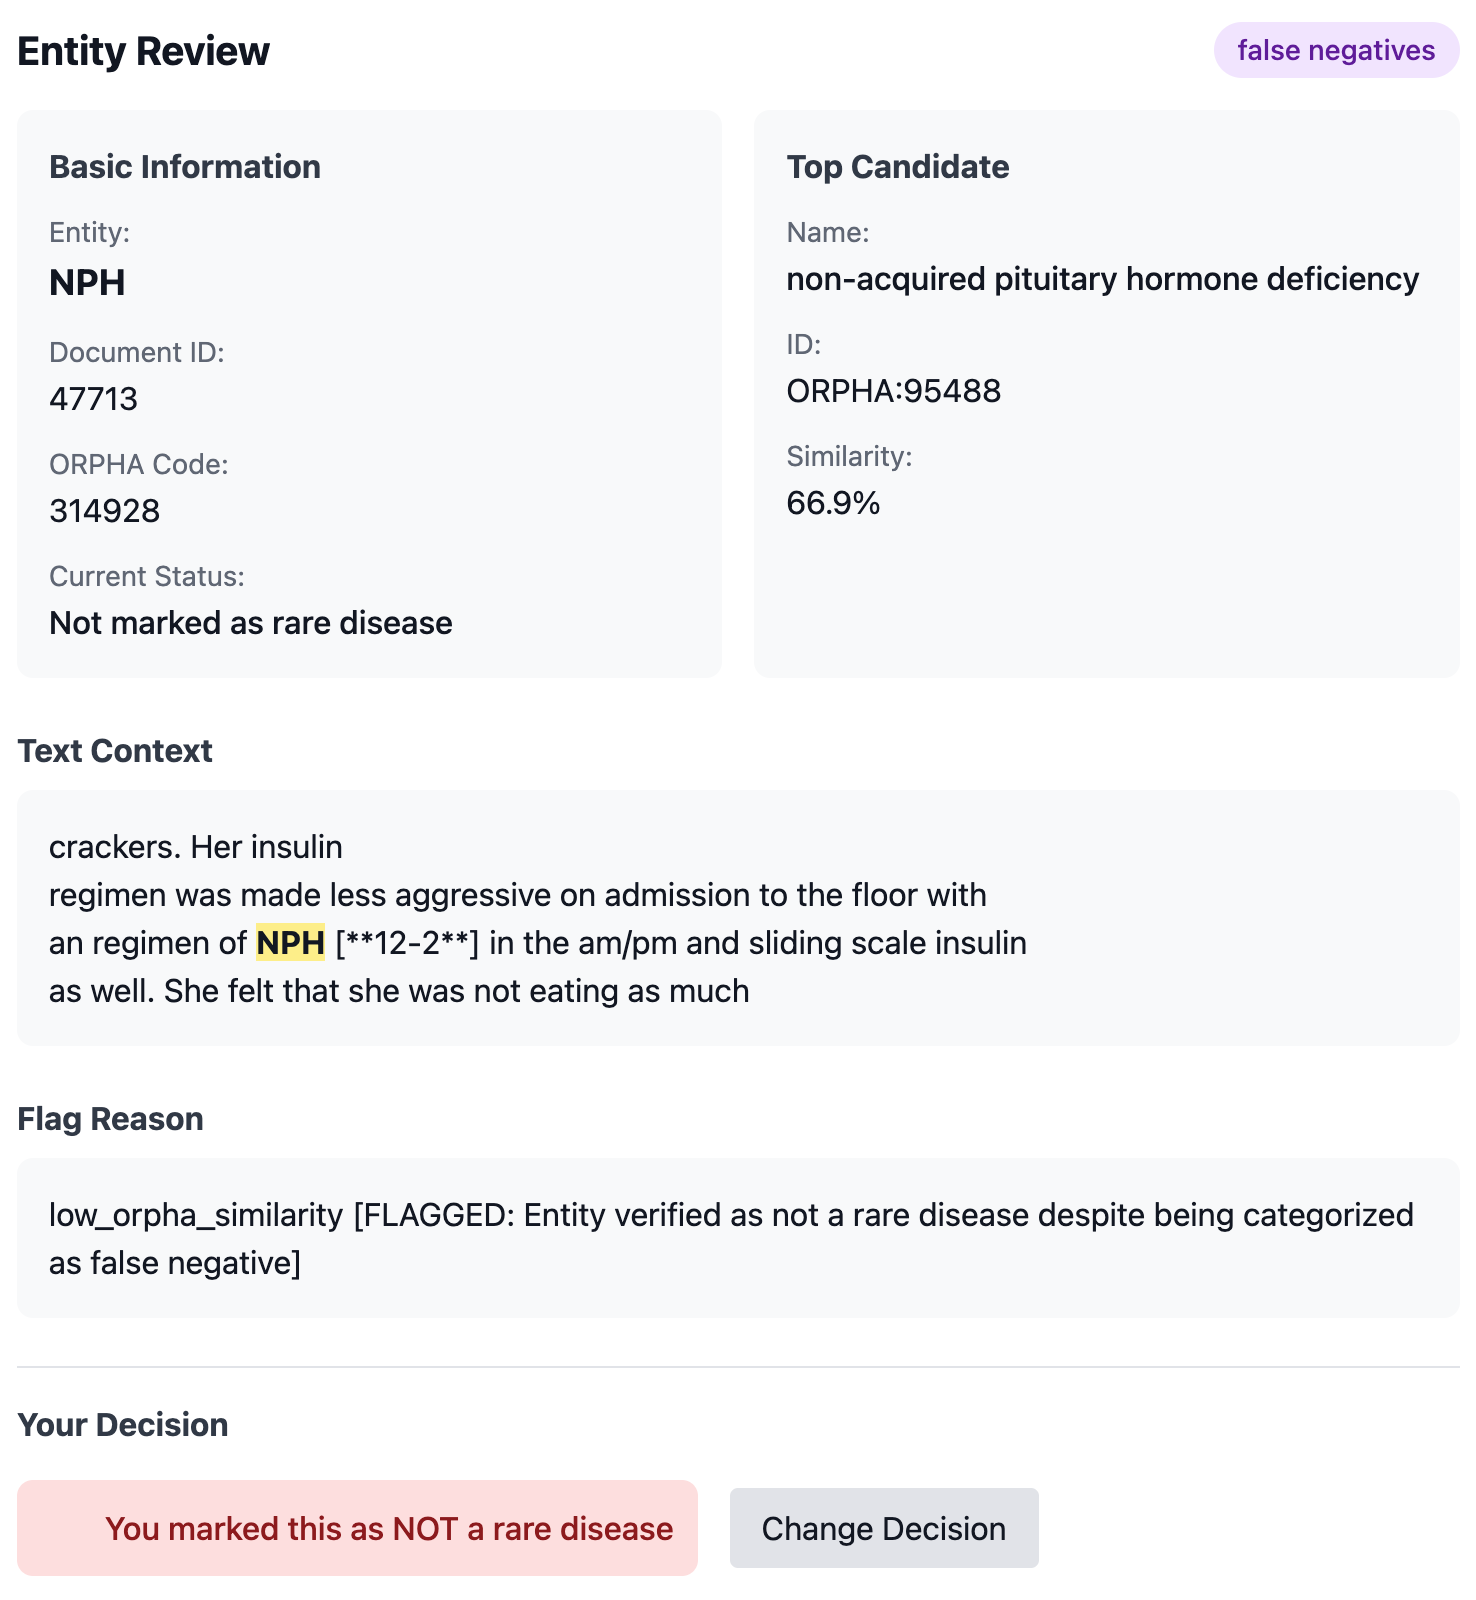
\includegraphics[width=1.0\textwidth]{figs/AnnotationUI.png}
%     \caption{\textbf{Example of Inappropriate Annotation in Noisy Dataset.} We note that while NPH as an abbreivation can be related to "normal pressure hydrocephalus" or other related conditions in the Orphanet ontology as annotated by \cite{dong2023ontology_poor_annotations}, NPH here in this context is actually referring to neutral protamine hagedorn, a type of insulin used to treat diabetes. }
%     \label{fig:ex_annotation}
% \end{figure}

% Run a blind experiment? MedStudent for comparison and review?

% \textbf{Baselines.} We investigate two rule-based approaches as they are substantially cheaper and easier to run. First, we attempt a simple embedding (MedEmbed \cite{balachandran2024medembed}) retrieval and string matching approach where we retrieve 20 candidates from HPO for each sentence and check if any retrieved entities are mentioned anywhere within the sentence or text. Second, we benchmarked the reported state of the art dictionary-based approach FastHPOCR \cite{groza2024fasthpocr} \cite{garcia2024_HPORAG}. 

% \textbf{RAG vs. RDMA.} We compare our approach across a plethora of models between the RAG-HPO and RDMA approaches. For model exploration, we explore biomedically finetuned models such as PhenoGPT \cite{yang2023enhancingphenotyperecognitionclinical}, BERT-based NER i2b2 \cite{rohanian2023lightweight_i2b2}, OpenBioLLM 3 70B \cite{OpenBioLLMs}, and general purpose models such as Llama 3.3 70B \cite{grattafiori2024llama3herdmodels}, Llama 3 70B \cite{grattafiori2024llama3herdmodels}, and the smaller Mistral 24B \cite{mistral2025small}.



% \input{sections/results/key_challenges}





% \input{sections/results/phenotype_mining}
% \input{sections/results/rd_mining}